\chapter{Multiple Integrals}

\section{Double Integrals over Rectangles}

\subsection*{Definition}
Definition The \textbf{double integral} of $f$ over the rectangle $R$ is
$$\iint\limits_R f(x,y)\:dA=\lim_{m,n\to\infty}\sum_{i=1}^m\sum_{j=1}^n f(x_{ij}^*,y_{ij}^*) \Delta A$$
if this limit exists.

If $f(x, y) \geq 0,$ then the volume V of the solid that lies above the rectangle $R$ and
below the surface $z = f(x, y)$ is
$$V=\iint\limits_R f(x,y)\:dA$$

\subsection*{Example}
Estimate the volume of the solid that lies above the square $R=[0,2]\times[0,2]$
and below the elliptic paraboloid $z=16-x^2-2y^2$. Divide R into four equal squares
and choose the sample point to be the upper right corner of each square $R_{ij}$.
Sketch the solid and the approximating rectangular boxes.

\subsection*{Solution}
The squares are shown below. The paraboloid is the graph of
$f(x,y)=16-x^2-2y^2$ and the area of each square is $\Delta A=1$. Approximating
the volume by the Riemann sum with $m=n=2$, we have
\begin{align*}
    V & \approx\sum_{i=1}^2\sum_{j=1}^2 f(x_i,y_j) \delta A          \\
      & =f(1,1)\delta A+f(1,2)\delta A+f(2,1)\delta A+f(2,2)\delta A \\
      & =13(1)+7(1)+10(1)+4(1)=34
\end{align*}
\begin{center}
    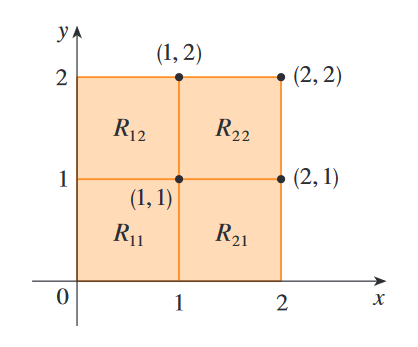
\includegraphics[scale=0.6]{example16-1-1.png}
\end{center}

We get better apprximations to the volume if we increase the number of squares.
Shown below is how the columns look more like the actual solid when we use 16, 64, and 256 squares.
\begin{center}
    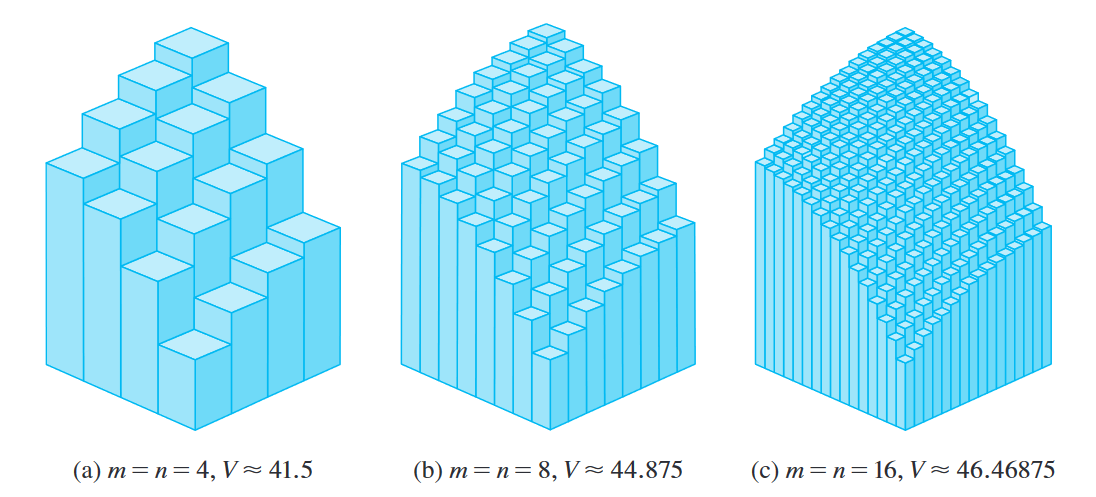
\includegraphics[scale=0.5]{example16-1-2.png}
\end{center}

\subsection*{Midpoint Rules for Double Integrals}
$$\iint\limits_R f(x,y)\:dA\approx\sum_{i=1}^m\sum_{j=1}^n f(\bar{x}_i,\bar{y}_j)\Delta A$$
where $\bar{x}_i$ is the midpoint of $[x_{i-1},x_i]$ and $\bar{y}_j$ is the midpoint
of $[y_{j-1},y_j]$.

\subsection*{Example}
Use the Midpoint Rule with $m=n=2$ to estimate the value of the integral
$\iint\limits_R (x-3y^2)\:dA$, where $R=\{(x,y)\:|\:0\leq x\leq 2, 1\leq y\leq 2\}$.

\subsection*{Solution}
In using the Midpoint Rule with $m=n=2$, we evaluate $f(x,y)=x-3y^2$ at the centers
of the four subrectangles shown below. So $\bar{x}_1=\frac{1}{2}$, $\bar{x}_2=\frac{3}{2}$,
$\bar{y}_1=\frac{5}{4}$, and $\bar{y}_2=\frac{7}{4}$. The area of each subrectangle
is $\Delta A=\frac{1}{2}$. Thus
\begin{align*}
    \iint\limits_R (x-3y^2)\:dA & \approx\sum_{i=1}^2\sum_{j=1}^2 f(\bar{x}_i,\bar{y}_j)\Delta A                                                                                                                           \\
                                & =f(\bar{x}_1,\bar{y}_1)\Delta A+f(\bar{x}_1,\bar{y}_2)\Delta A+f(\bar{x}_2,\bar{y}_1)\Delta A+f(\bar{x}_2,\bar{y}_2)\Delta A                                                             \\
                                & =f\left(\frac{1}{2},\frac{5}{4}\right)\Delta A+f\left(\frac{1}{2},\frac{7}{4}\right)\Delta A+f\left(\frac{3}{2},\frac{5}{4}\right)\Delta A+f\left(\frac{3}{2},\frac{7}{4}\right)\Delta A \\
                                & =\left(-\frac{67}{16}\right)\frac{1}{2}+\left(-\frac{139}{16}\right)\frac{1}{2}+\left(-\frac{51}{16}\right)\frac{1}{2}+\left(-\frac{123}{16}\right)\frac{1}{2}                           \\
                                & =-\frac{95}{8}=-11.875
\end{align*}
Thus we have
$$\iint\limits_R (x-3y^2)\:dA\approx -11.875$$

\subsection*{Average Value}
The average value of a function $f$ of one variable is
$$f_{ave}=\frac{1}{b-a}\int_a^b f(x)\:dx$$
Similarly, the \textbf{average value} of a function $f$ of two variables defined on
a rectangle $R$ is
$$f_{ave}=\frac{1}{A(R)}\iint\limits_R f(x,y)\:dA$$
where $A(R)$ is the area of $R$.

\section{Iterated Integrals}

\subsection*{Example}
Evaluate the iterated integrals.
\begin{enumerate}[(a)]
    \item $\int_0^3 \int_1^2 x^2y\:dy\:dx$
    \item $\int_1^2 \int_0^3 x^2y\:dx\:dy$
\end{enumerate}

\subsection*{Solution}
\begin{enumerate}[(a)]
    \item Regarding $x$ as a constant, we obtain
          $$\int_1^2 x^2y\:dy=\left[x^2\frac{y^2}{2}\right]_{y=1}^{y=2}$$
          $$=x^2\left(\frac{2^2}{2}\right)-x^2\left(\frac{1^2}{2}\right)=\frac{3}{2}x^2$$
          Thus, the function $A$ in the preceding discussion is given by $A(x)=\frac{3}{2}x^2$
          in this example. We now integrate this function of $x$ from 0 to 3:
          $$\int_0^3 \int_1^2 x^2y\:dy\:dx=\int_0^3\left[\int_1^2 x^2y\:dy\right]\:dx$$
          $$=\int_0^3 \frac{3}{2}x^2\:dx=\left[\frac{x^3}{2}\right]_0^3=\frac{27}{2}$$
    \item Here we first integrate with respect to $x$:
          $$\int_1^2 \int_0^3 x^2y\:dx\:dy=\int_1^2\left[\int_0^3 x^2y\:dx\right]\:dy=
              \int_1^2\left[\frac{x^3}{3}y\right]_{x=0}^{x=3}\:dy$$
          $$=\int_1^2 9y\:dy=\left[9\frac{y^2}{2}\right]_1^2=\frac{27}{2}$$
          Notice that we obtained the same answer whether we integrated with respect to
          $y$ or $x$ first. The order of integration doesn't matter.
\end{enumerate}

\subsection*{Fubini's Theorem}
If $f$ is continuous on the rectangle $R=\{(x,y)\:|\:a\leq x\leq b,\: c\leq y\leq d\}$ then
$$\iint\limits_R f(x,y)\: dA=\int_a^b\int_c^d f(x,y)\:dy\:dx=\int_c^d\int_a^b f(x,y)\:dx\:dy$$
More generally, this is true if we assume that $f$ is bounded on $R$, $f$ is discontinuous
only on a finite number of smooth curves, and the iterated integrals exist.

\subsection*{Example}
If $R=[0,\pi/2]\times[0,\pi/2]$, then
$$\iint\limits_R \sin{x}\cos{y}\:dA=\int_0^{\pi/2}\sin{x}\:dx\int_0^{\pi/2}\cos{y}\:dy$$
$$=[-\cos{x}]_0^{\pi/2}[\sin{y}]_0^{\pi/2}=1\cdot 1=1$$
\begin{center}
    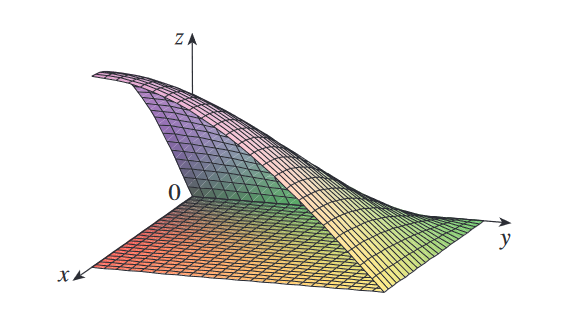
\includegraphics[scale=0.6]{example16-2-1.png}
\end{center}

\section{Double Integrals over General Regions}

If $F$ is integrable over $R$, then we define the \textbf{double integral of $f$ over $D$} by
$$\iint\limits_D f(x,y)\:dA=\iint\limits_R F(x,y)\:dA$$

If $f$ is continuous on a type I region $D$ such that
$$D=\left\{(x,y)\:|\: a\leq x\leq b,|\: g_1(x)\leq y\leq g_2(x)\right\}$$
then
$$\iint\limits_D f(x,y)\:dA=\int_a^b\int_{g_1(x)}^{g_2(x)}f(x,y)\:dy\:dx$$

Using the same methods as above, we can show that
$$\iint\limits_D f(x,y)\:dA=\int_c^d\int_{h_1(y)}^{h_2(y)}f(x,y)\:dx\:dy$$
where $D$ is a type II region.

\subsection*{Example}
Evaluate $\int\limits_D (x+2y)\:dA$, where $D$ is the region bounded by the parabolas
$y=2x^2$ and $y=1+x^2$

\subsection*{Solution}
The parabolas intersect when $2x^2=1+x^2$, that is, $x^2=1$, so $x=\pm 1$. We note
that the region $D$, is a type I region but not a type II region and we can write
$$D=\{(x,y)\:|\: -1\leq x\leq 1,\: 2x^2\leq y\leq 1+x^2\}$$
Since the lower boundary is $y=2x^2$ and the upper boundary is $y=1+x^2$, we have
\begin{align*}
    \iint\limits_D(x+2y)\:dA & =\int_{-1}^1\int_{2x^2}^{1+x^2} (x+2y)\:dy\:dx                                                  \\
                             & =\int_{-1}^1\left[xy+y^2\right]_{y=2x^2}^{y=1+x^2}\:dx                                          \\
                             & =\int_{-1}^1\left[x(1+x^2)+(1+x^2)^2-x(2x^2)-(2x^2)^2\right]\:dx                                \\
                             & =\int_{-1}^1(-3x^4-x^3+2x^2+x+1)\:dx                                                            \\
                             & =\left[-3\frac{x^5}{5}-\frac{x^4}{4}+2\frac{x^3}{3}+\frac{x^2}{2}+x\right]_{-1}^1=\frac{32}{15}
\end{align*}

\subsection*{Example}
Evaluate $\iint\limits_D xy\:dA$, where $D$ is the region bounded by the line $y=x-1$
and the parabola $y^2=2x+6$.

\subsection*{Solution}
The region $D$ is shown below. Again $D$ is both type I and type II, but the description of $D$ as a type I region is
more complicated because the lower boundary consists of two parts. Therefore, we prefer
to express $D$ as a type II region:
$$D=\{(x,y)\:|\:-2\leq y\leq 4,\: \frac{1}{2}y^2-3\leq x\leq y+1\}$$
\begin{center}
    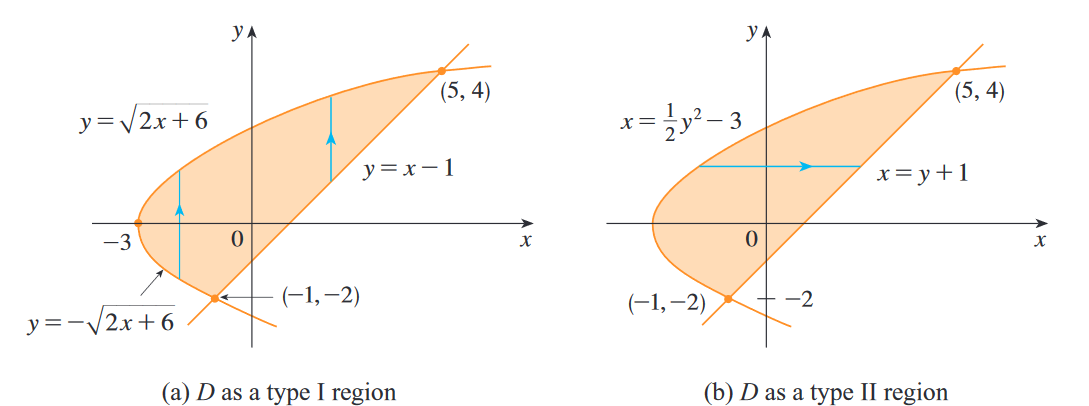
\includegraphics[scale=0.5]{example16-3-1.png}
\end{center}
\begin{align*}
    \iint\limits_D xy\:dA & =\int_{-2}^4\int_{\frac{1}{2}y^2-3}^{y+1}xy\:dx\:dy=\int_{-2}^4\left[\frac{x^2}{2}y\right]_{x=\frac{1}{2}y^2-3}^{x=y+1}\:dy \\
                          & =\frac{1}{2}\int_{-2}^4 y[(y+1)^2-(\frac{1}{2}y^2-3)^2]\:dy                                                                 \\
                          & =\frac{1}{2}\int_{-2}^4 \left(-\frac{y^5}{4}+4y^3+2y^2-8y\right)\:dy                                                        \\
                          & =\frac{1}{2}\left[-\frac{y^6}{24}+y^4+2\frac{y^3}{3}-4y^2\right]_{-2}^4=36
\end{align*}
If we had expressed $D$ as a type I region using (a), then we would have obtained
$$\iint\limits_D xy\: dA=\int_{-3}^{-1}\int_{-\sqrt{2x+6}}^{\sqrt{2x+6}} xy\:dy\:dx+
    \int_{-1}^5\int_{x-1}^{\sqrt{2x+6}} xy\:dy\:dx$$
but this would have involved more work than the other method.

\subsection*{Properties of Double Integrals}
\begin{enumerate}
    \item[(6)] $\iint\limits_D [f(x,y)+g(x,y)]\:dA=\iint\limits_D f(x,y)\:dA+\iint\limits_D g(x,y)\:dA$
    \item[(7)] $\iint\limits_D cf(x,y)\:dA=c\iint\limits_D f(x,y)\:dA$
    \item[(9)] $\iint\limits_D f(x,y)\:dA=\iint\limits_{D_1} f(x,y)\:dA+\iint\limits_{D_2} f(x,y)\:dA$
    \item[(10)] $\iint\limits_D 1\:dA=A(D)$
    \item[(11)] If $m\leq f(x,y)\leq M$ for all $(x,y)$ in $D$, then $$mA(D)\leq\iint\limits_D f(x,y)\:dA\leq MA(D)$$
\end{enumerate}

\subsection*{Example}
Use Property 11 to estimate the integral $\iint\limits_D e^{\sin{x}\cos{y}}\:dA$,
where $D$ is the disk with center the origin and radius 2.

\subsection*{Solution}
Since $-1\leq\sin{x}\leq 1$ and $-1\leq \cos{y}\leq 1$, we have $-1\leq\sin{x}\cos{y}\leq 1$
and therefore
$$e^{-1}\leq e^{\sin{x}\cos{y}}\leq e^1=e$$
Thus, using $m=e^{-1}=1/e$, $M=e$, and $A(D)=\pi(2)^2$ in Property 11, we obtain
$$\frac{4\pi}{e}\leq\iint\limits_D e^{\sin{x}\cos{y}}\:dA\leq 4\pi e$$

\section{Double Integrals in Polar Coordinates}

\subsection*{Change to Polar Coordinates in a Double Integral}
If $f$ is continuous on a polar rectangle $R$ given by $0\leq a\leq r\leq b$,
$\alpha\leq\theta\leq\beta$, where $0\leq\beta-\alpha\leq 2\pi$, then
$$\iint\limits_R f(x,y)\:dA=\int_\alpha^\beta\int_a^b f(r\cos{\theta},r\sin{\theta})\:r\:dr\:d\theta$$

\subsection*{Example}
Find the volume of the solid bounded by the plane $z=0$ and the paraboloid $z=1-x^2-y^2$.

\subsection*{Solution}
If we put $z=0$ in the equation of the paraboloid, we get $x^2+y^2=1$. This means that
the plane intersects the paraboloid in the circle $x^2+y^2=1$, so the solid lies under
the paraboloid and above the circular disk $D$ given by $x^2+y^2\leq 1$. In polar
coordinates $D$ is given by $0\leq r\leq 1$, $0\leq\theta\leq 2\pi$ Since
$1-x^2-y^2=1-r^2$, the volume is
\begin{align*}
    V & =\iint\limits_D (1-x^2-y^2)\:dA=\int_0^{2\pi}\int_0^1 (1-r^2)\:r\:dr\:d\theta                             \\
      & =\int_0^{2\pi}\:d\theta\int_0^1(r-r^3)\:dr=2\pi\left[\frac{r^2}{2}-\frac{r^4}{4}\right]_0^1=\frac{\pi}{2}
\end{align*}
If we had used rectangular coordinates instead of polar coordinates, then we would have obtained
$$V=\iint\limits_D(1-x^2-y^2)\:dA=\int_{-1}^1\int_{-\sqrt{1-x^2}}^{\sqrt{1-x^2}}
    (1-x^2-y^2)\:dy\:dx$$
which is not easy to evaluate because it involves finding the following integrals:
$$\int\sqrt{1-x^2}\:dx \qquad \int x^2\sqrt{1-x^2}\:dx \qquad \int(1-x^2)^{3/2}\:dx$$

If $f$ is continuous on the polar region of the form
$$D=\left\{(r,\theta)\:|\:\alpha\leq\theta\beta,\: h_1(\theta)\leq r\leq h_2(\theta)\right\}$$
then
$$\iint\limits_D f(x,y)\:dA=\int_\alpha^\beta\int_{h_1(\theta)}^{h_2(\theta)}
    f(r\cos{\theta}, r\sin{\theta})\:r\:dr\:d\theta$$

\subsection*{Example}
Use a double integral to find the area enclosed by one loop of the four-leaved rose
$r=\cos{2\theta}$.
\begin{center}
    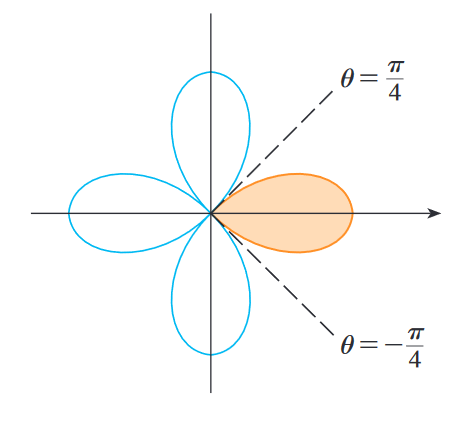
\includegraphics[scale=0.5]{example16-4-1.png}
\end{center}

\subsection*{Solution}
We see that the loop is given by the region
$$D=\{(r,\theta)\:|\:-\pi/4\leq\theta\leq\pi/4.\:0\leq r\leq\cos{2\theta}\}$$
So the area is
\begin{align*}
    A(D) & =\iint\limits_D dA=\int_{-\pi/4}^{\pi/4}\int_0^{\cos{2\theta}}r\:dr\:d\theta                                                                       \\
         & =\int_{-\pi/4}^{\pi/4}\left[\frac{1}{2}r^2\right]_0^{\cos{2\theta}}d\theta=\frac{1}{2}\int_{-\pi/4}^{\pi/4} \cos^2{2\theta}\:d\theta               \\
         & =\frac{1}{4}\int_{-\pi/4}^{\pi/4}(1+\cos{4\theta})\:d\theta=\frac{1}{4}\left[\theta+\frac{1}{4}\sin{4\theta}\right]_{-\pi/4}^{\pi/4}=\frac{\pi}{8}
\end{align*}

\section{Applications of Double Integrals}

\subsection*{Density and Mass}
$$\rho(x,y)=\lim\frac{\Delta m}{\Delta A}$$
$$m=\lim_{k,l\to\infty}\sum_{i=1}^k\sum_{j=1}^l\rho(x_{ij}^*,y_{ij}^*)\Delta A=
    \iint\limits_D\rho(x,y)\:dA$$

\subsection*{Example}
Charge is distributed over the triangular region $D$ in the figure so that the charge
density at $(x,y)$ is $\sigma(x,y)=xy$, measured in coulombs per square meter
$(\text{C/m}^2)$. Find the total charge.

\subsection*{Solution}
\begin{align*}
    Q & =\iint_D \sigma(x,y)\:dA=\int_0^1\int_{1-x}^1 xy\:dy\:dx                                                 \\
      & =\int_0^1\left[x\frac{y^2}{2}\right]_{y=1-x}^{y=1}dx=\int_0^1\frac{x}{2}[1^2-(1-x)^2]\:dx                \\
      & =\frac{1}{2}\int_0^1(2x^2-x^3)\:dx=\frac{1}{2}\left[\frac{2x^3}{3}-\frac{x^4}{4}\right]_0^1=\frac{5}{24}
\end{align*}
Thus the total charge is $\frac{5}{24}$ C.

\subsection*{Moments and Centers of Mass}
The \textbf{moment} of the entire lamina \textbf{about the $x$-axis}:
$$M_x=\lim_{m,n\to\infty}\sum_{i=1}^m\sum_{j=1}^n y_{ij}^*\rho(x_{ij}^*,y_{ij}^*)\Delta A=
    \iint\limits_D y\rho(x,y)\:dA$$
Similarly, the \textbf{moment about the $y$-axis} is:
$$M_y=\lim_{m,n\to\infty}\sum_{i=1}^m\sum_{j=1}^n x_{ij}^*\rho(y_{ij}^*,x_{ij}^*)\Delta A=
    \iint\limits_D x\rho(x,y)\:dA$$
The coordinates $(\bar{x},\bar{y})$ of the center of mass of a lamina occupying the region
$D$ and having density function $\rho(x,y)$ are
$$\bar{x}=\frac{M_y}{m}=\frac{1}{m}\iint\limits_D x\rho(x,y)\:dA \qquad
    \bar{y}=\frac{M_x}{m}=\frac{1}{m}\iint\limits_D y\rho(x,y)\:dA$$
where the mass $m$ is given by
$$m=\iint\limits_D \rho(x,y)\:dA$$

\subsection*{Moment of Inertia}
The \textbf{moment of inertia} of the lamina \textbf{about the $x$-axis}:
$$I_x=\lim_{m,n\to\infty}\sum_{i=1}^m\sum_{j=1}^n(y_{ij}^*)^2\rho(x_{ij}^*,y_{ij}^*)\Delta A=
    \iint\limits_D y^2\rho(x,y)\:dA$$
Similarly, the \textbf{moment of inertia about the $y$-axis} is:
$$I_y=\lim_{m,n\to\infty}\sum_{i=1}^m\sum_{j=1}^n(x_{ij}^*)^2\rho(y_{ij}^*,x_{ij}^*)\Delta A=
    \iint\limits_D x^2\rho(x,y)\:dA$$
It is also of interest to consider the \textbf{moment of inertia about the origin}, also
called the \textbf{polar moment of inertia}:
$$I_0=\lim_{m,n\to\infty}\sum_{i=1}^m\sum_{j=1}^n\left[(x_{ij}^*)^2+(y_{ij}^*)^2\right]
    \rho(x_{ij}^*,y_{ij}^*)\Delta A=\iint\limits_D(x^2+y^2)\rho(x,y)\:dA$$
Note that $I_0=I_x+I_y$.

\subsection*{Example}
Find the moments of inertia $I_x$, $I_y$, and $I_0$ of a homogeneous disk $D$ with density
$\rho(x,y)=\rho$ center the origin, and radius $a$.

\subsection*{Solution}
The boundary of $D$ is the circle $x^2+y^2=a^2$ and in polar coordinates $D$ is
described by $0\leq\theta\leq 2\pi$, $0\leq r\leq a$. Let's compute $I_0$ first:
$$I_0=\iint\limits_D(x^2+y^2)\rho\:dA=\rho\int_0^{2\pi}\int_0^{a}r^2r\:dr\:d\theta$$
$$\rho\int_0^{2\pi}d\theta\int_0^ar^3\:dr=2\pi\rho\left[\frac{r^4}{4}\right]_0^a=\frac{\pi\rho a^4}{2}$$
Instead of computing $I_x$ and $I_y$ directly, we use the facts that $I_x+I_y=I_0$ and
$I_x=I_y$ (from the symmetry of the problem). Thus
$$I_x=I_y=\frac{I_0}{2}=\frac{\pi\rho a^4}{4}$$

\subsection*{Example}
The manager of a movie theater determines that the average time movie-goers
wait in line to buy a ticket for this week’s film is 10 minutes and the average
time they wait to buy popcorn is 5 minutes. Assuming that the waiting times are
independent, find the probability that a moviegoer waits a total of less than 20
minutes before taking his or her seat.

\subsection*{Solution}
Assuming that both the waiting time $X$ for the ticket purchase and the waiting time
$Y$ in the refreshment line are modeled by exponential probability density functions,
we can write the individual density functions as
\[
    f_1(x) =
    \begin{cases}
        0                     & \text{if $x<0$}     \\
        \frac{1}{10}e^{-x/10} & \text{if $x\geq 0$}
    \end{cases} \qquad
    f_2(x) =
    \begin{cases}
        0                   & \text{if $y<0$}     \\
        \frac{1}{5}e^{-y/5} & \text{if $y\geq 0$}
    \end{cases}
\]
Since $X$ and $Y$ are independent, the joint density function is the product:
\[
    f(x,y)=f_1(x)f_2(y)=
    \begin{cases}
        \frac{1}{5}e^{-x/10}e^{-y/5} & \text{if $x\geq 0$, $y\geq 0$} \\
        0                            & \text{otherwise}
    \end{cases}
\]
We are asked for the probability that $X+Y<20$:
$$P(X+Y<20)=P((X,Y)\in D)$$
where $D$ is the triangular region given by the area under $y=-x+20$. Thus
\begin{align*}
    P(X+Y<20) & =\iint\limits_D f(x,y)\:dA=\int_0^{20}\int_0^{20-x}\frac{1}{50}e^{-x/10}e^{-y/5}\:dy\:dx \\
              & =\frac{1}{50}\int_0^{20}\left[e^{-x/10}(-5)e^{-y/5}\right]_{y=0}^{y=20-x}\:dx            \\
              & =\frac{1}{10}\int_0^{20}e^{-x/10}(1-e^{(x-20)/5})\:dx                                    \\
              & =\frac{1}{10}\int_0^{20}(e^{-x/10}-e^{-4}e^{x/10})\:dx                                   \\
              & =1+e^{-4}-2e^{-2}\approx 0.7476
\end{align*}
This means that about 75\% of the moviegoers wait less than 20 minutes before taking
their seats.

\section{Surface Area}
We define the \textbf{surface area} of $S$ to be
\begin{align*}
    A(S) & =\lim_{m,n\to\infty}\sum_{i=1}^m\sum_{j=1}^n \Delta T_{ij}                                       \\
         & =\lim_{m,n\to\infty}\sum_{i=1}^m\sum_{j=1}^n\sqrt{[f_x(x_i,y_j)]^2+[f_y(x_i,y_j)]^2+1}\:\Delta A
\end{align*}

The area of the surface with equation $z=f(x, y), (x, y)\in D$,
where $f_x$ and $f_y$ are continuous, is
$$A(S)=\iint\limits_D\sqrt{[f_x(x_i,y_j)]^2+[f_y(x_i,y_j)]^2+1}\:\Delta A)$$

Rewrite it as follows
$$A(S)=\iint\limits_D\sqrt{1+\left(\pdv{z}{x}\right)^2+\left(\pdv{z}{y}\right)^2}\:dA$$

\subsection*{Example}
Find the surface area of the part of the surface $z=x^2+2y$ that lies above the triangular
region $T$ in the $xy$-plane with the vertices $(0,0)$, $(1,0)$, and $(1,1)$.

\subsection*{Solution}
The region $T$ is described by
$$T={(x,y)\:|\:0\leq x\leq 1,\: 0\leq y\leq x}$$
Using $f(x,y)=x^2+2y$, we get
\begin{align*}
    A & =\iint\limits_T \sqrt{(2x)^2+(2)^2+1}\:dA=\int_0^1\int_0^x\sqrt{4x^2+5}\:dy\:dx                                    \\
      & =\int_0^1 x\sqrt{4x^2+5}\:dx=\left[\frac{1}{8}\cdot\frac{2}{3}(4x^2+5)^{3/2}\right]_0^1=\frac{1}{12}(27-5\sqrt{5})
\end{align*}

The figure below shows the portion of the surface whose area we have just computed.
\begin{center}
    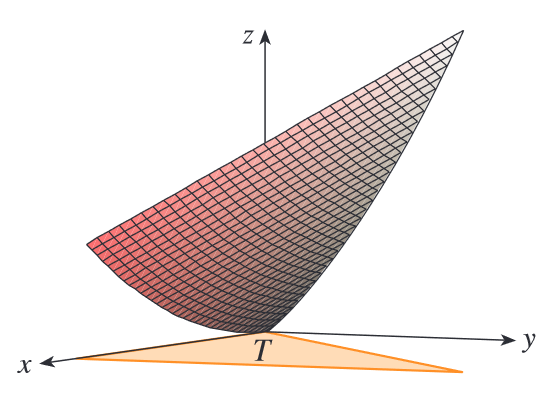
\includegraphics[scale=0.5]{example16-5-1.png}
\end{center}

\section{Triple Integrals}

\subsection*{Definition}
The \textbf{triple integral} of $f$ over the box $B$ is
$$\iiint\limits_B f(x,y,z)\:dV=\lim_{l,m,n\to\infty}\sum_{i=1}^l\sum_{j=1}^m\sum_{k=1}^n
    f(x_{ijk}^*,y_{ijk}^*,z_{ijk}^*)\Delta V$$

\subsection*{Fubini's Theorem for Triple Integrals}
If $f$ is continuous on the rectangular box $B=[a,b]\times[c,d]\times[r,s]$, then
$$\iiint\limits_B f(x,y,z)\:dV=\int_r^s\int_c^d\int_a^b f(x,y,z)\:dx\:dy\:dz$$

\subsection*{Example}
Evaluate $\iiint\limits_E z\:dV$, where $E$ is the solid tetrahedron bounded by the
four planes $x=0$, $y=0$, $z=0$, and $x+y+z=1$.

\subsection*{Solution}
When we set up a triple integral it's wise to draw \textbf{two} diagrams: one of the
solid region $E$ and one of its projection $D$ on the $xy$-plane. The lower boundary
of the tetrahedron is the plane $z=0$ and the upper boundary is the plane $x+y+z=1$,
so we use $u_1(x,y)=$ and $u_2(x,y)=1-x-y$. Notice that the planes $x+y+z=1$ and $z=0$
intersect in the line $x+y=1$ in the $xy$-plane. So the projection of $E$ is the triangular
region and we have
$$E=\{(x,y,z)\:|\:0\leq x\leq 1,\:0\leq y\leq 1-x,\:0\leq z\leq 1-x-y\}$$
This description of $E$ as a type I region enables us to evaluate the integral as follows:
\begin{align*}
    \iiint\limits_E z\:dV & =\int_0^1\int_0^{1-x}\int_0^{1-x-y}z\:dz\:dy\:dx=\int_0^1\int_0^{1-x}\left[\frac{z^2}{2}\right]_{z=0}^{z=1-x-y}dy\:dx  \\
                          & =\frac{1}{2}\int_0^1\int_0^{1-x}(1-x-y^2)\:dy\:dx=\frac{1}{2}\int_0^1\left[-\frac{(1-x-y)^3}{3}\right]_{y=0}^{y=1-x}dx \\
                          & =\frac{1}{6}\int_0^1(1-x)^3\:dx=\frac{1}{6}\left[-\frac{(1-x)^4}{4}\right]_0^1=\frac{1}{24}
\end{align*}

\subsection*{Applications of Triple Integrals}
The case where $f(x,y,z)=1$ for all points in $E$, the triple integral represents the volume of $E$:
$$V(E)=\iiint\limits_E dV$$

\subsection*{Example}
Use a triple integral to find the volume of the tetrahedron $T$ bounded by the planes
$x+2y+z=2$, $x=2y$, $x=0$, and $z=0$.

\subsection*{Solution}
The tetrahedron $T$ and its projection $D$ on the $xy$-plane are shown below. The
lower boundary of $T$ is the plane $z=0$ and the upper boundary is the plane $x+2y+z=2$,
that is, $z=2-x-2y$.
\begin{center}
    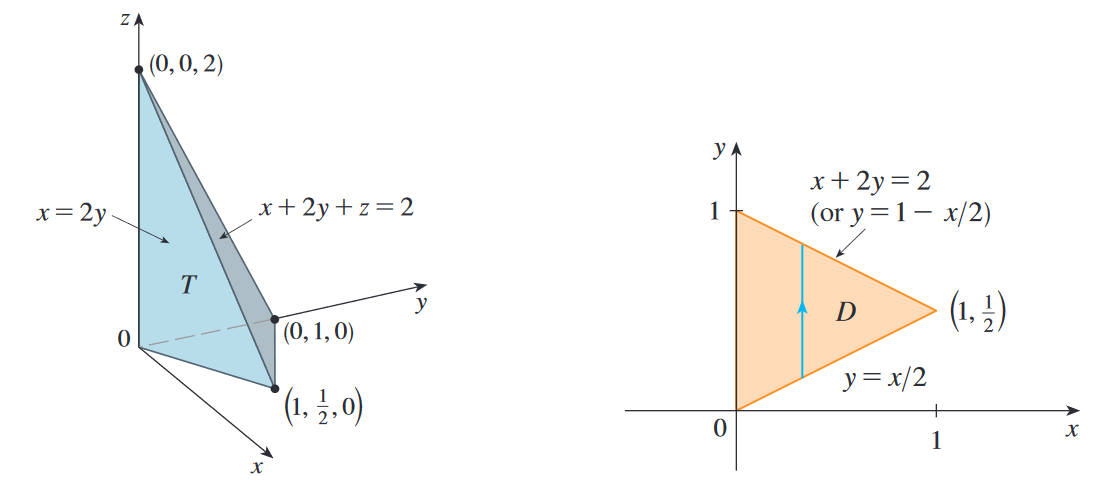
\includegraphics[scale=0.5]{example16-7-1.png}
\end{center}
Therefore, we have
$$V(T)=\iiint\limits_T dV=\int_0^1\int_{x/2}^{1-x/2}\int_0^{2-x-2y}dz\:dy\:dx$$
$$=\int_0^1\int_{x/2}^{1-x/2}(2-x-2y)\:dy\:dx=\frac{1}{3}$$

\section{Triple Integrals in Cylindrical and Spherical Coordinates}

\subsection*{Cylindrical Coordinates}
To convert form cylindrical to rectangular coordinates, we use the equations
$$x=r\cos{\theta} \qquad y=r\sin{\theta} \qquad z=z$$
whereas to convert from rectangular to cylindrical coordinates, we use
$$r^2=x^2+y^2 \qquad \tan{\theta}=\frac{y}{x} \qquad z=z$$

\subsection*{Triple Integration in Cylindrical Coordinates}
$$\iiint\limits_E f(x,y,z)\:dV=\int_\alpha^\beta\int_{h_1(\theta)}^{h_2(\theta)}
    \int_{u_1(r\cos{\theta}, r\sin{\theta})}^{u_2(r\cos{\theta}, r\sin{\theta})}
    f(r\cos{\theta}, r\sin{\theta}, z)\:r\:dz\:dr\:d\theta$$

\subsection*{Example}
A solid $E$ lies within the cylinder $x^2+y^2=1$, below the plane $z=4$, and above
the paraboloid $z=1-x^2-y^2$. The density at any point is proportional to its distance
from the axis of the cylinder. Find the mass of $E$.

\subsection*{Solution}
In cylindrical coordinates the cylinder is $r=1$ and the paraboloid is $z=1-r^2$,
so we can write
$$E=\{(r,\theta,z)\:|\:0\leq\theta\leq 2\pi,\:0\leq r\leq 1,\: 1-r^2\leq z\leq 4\}$$
Since the density at $(x,y,z)$ is proportional to the distance from the $z$-axis, the
density function is
$$f(x,y,z)=K\sqrt{x^2+y^2}=Kr$$
where $K$ is the proportionality constant. Therefore, the mass of $E$ is
$$m=\iiint\limits_E K\sqrt{x^2+y^2}\:dV=\int_0^{2\pi}\int_0^1\int_{1-r^2}^4(Kr)\:r\:dz\:dr\:d\theta$$
$$=\int_0^{2\pi}\int_0^1 Kr^2[4-(1-r^2)]\:dr\:d\theta=K\int_0^{2\pi} d\theta\int_0^1(3r^2+r^4)\:dr$$
$$=2\pi K\left[r^3+\frac{r^5}{5}\right]_0^1=\frac{12\pi K}{5}$$

\subsection*{Spherical Coordinates}
To convert from spherical to rectangular coordinates, we use the eqations
$$x=\rho\sin{\phi}\cos{\theta} \qquad y=\rho\sin{\phi}\sin{\theta} \qquad z=\rho\cos{\phi}$$
Also, the distance formula shows that
$$\rho^2=x^2+y^2+z^2$$

\subsection*{Triple Integration in Spherical Coordinates}
$\iiint\limits_E f(x,y,z)\:dV$
$$=\int_c^d\int_\alpha^\beta\int_a^b f(\rho\sin{\phi}\cos{\theta},
    \rho\sin{\phi}\sin{\theta},\rho\cos{\phi})\:\rho^2\sin{\phi}\:d\rho\:d\theta\:d\phi$$
where E is a spherical wedge given by
$$E=\{(\rho,\theta,\phi)\:|\:a\leq\rho\leq b,\: \alpha\leq\theta\leq\beta,\:c\leq\phi\leq d\}$$

\subsection*{Example}
Evaluate $\iiint\limits_B e^{(x^2+y^2+z^2)^{3/2}}dV$, where $B$ is the unit ball:
$$B=\{(x,y,z)\:|\: x^2+y^2+z^2\leq 1\}$$

\subsection*{Solution}
Since the boundary of $B$ is a sphere, we use spherical coordinates:
$$B=\{(\rho,\theta,\phi)\:|\:0\leq\rho\leq 1,\: 0\leq\theta\leq 2\pi,\:0\leq\phi\leq\pi\}$$
In addition, spherical coordinates are appropriate because
$$x^2+y^2+z^2=\rho^2$$
Thus
$$\iiint\limits_B e^{(x^2+y^2+z^2)^{3/2}}dV=\int_0^\pi\int_0^{2\pi}\int_0^1 e^{(\rho^2)^{3/2}}
    \rho^2\sin{\phi}\:d\rho\:d\theta\:d\phi$$
$$=\int_0^\pi\sin{\phi}\:d\phi\int_0^{2\pi}d\theta\int_0^1\rho^2e^{\rho^3}\:d\rho$$
$$=\left[-\cos{\phi}\right]_0^\pi (2\pi)\left[\frac{1}{3}e^{\rho^3}\right]_0^1=\frac{4}{3}\pi(e-1)$$

\section{Change of Variables in Multiple Integrals}

\subsection*{Example}
A transformation is defined by the equations
$$x=u^2-v^2 \qquad y=2uv$$
Find the image of the square $S=\{(u,v)\:|\:0\leq u\leq 1,\: 0\leq v\leq 1\}$.

\subsection*{Solution}
The transformation maps the boundary of $S$ into the boundary of the image.
So we begin by finding the images of the sides of $S$. The first side, $S_1$,
is given by $v=0$ $(0\leq u\leq 1)$. From the given equations we have $x=u^2$, $y=0$,
and so $0\leq x\leq 1$. Thus $S_1$ is mapped onto the line segment from (0,0) to (1,0)
in the $xy$-plane. The second side, $S_2$, is $u=1$ $(0\leq v\leq 1)$ and, putting
$u=1$ in the given equations, we get
$$x=1-v^2 \qquad y=2v$$
Eliminating $v$, we obtain
$$x=1-\frac{y^2}{4} \qquad 0\leq x\leq 1$$
which is part of a parabola. Similarly, $S_3$ is given by $v=1$ $(0\leq u\leq 1)$, whose
image is the parabolic arc
$$x=\frac{y^2}{4}-1 \qquad -1\leq x\leq 0$$
Finally, $S_4$ is given by $u=0$ $(0\leq v\leq 1)$ whose image is $x=-v^2$, $y=0$,
that is, $-1\leq x\leq 0$. The image of $S$ is the region $R$ bounded by the $x$-axis
and the parabolas given by the two equations we found.

\subsection*{Definition}
The \textbf{Jacobian} of the transformation $T$ given by $x=g(u,v)$ and $y=h(u,v)$ is
$$\pdv{(x,y)}{(u,v)}=
    \begin{vmatrix}
        \dfrac{\partial x}{\partial u} & \dfrac{\partial x}{\partial v} \\[1em]
        \dfrac{\partial y}{\partial u} & \dfrac{\partial y}{\partial v}
    \end{vmatrix}
    =\pdv{x}{u}\pdv{y}{v}-\pdv{x}{v}\pdv{y}{u}$$

\subsection*{Change of Variables in a Double Integral}
Suppose that $T$ is a $C^1$ transformation whose Jacobian is nonzero and that $T$
maps a region $S$ in the $uv$-plane onto a region $R$ in the $xy$-plane. Suppose
that $f$ is continuous on $R$ and that $R$ and $S$ are type I or type II plane regions.
Suppose also that $T$ is one-to-one, except perhaps on the boundary of $S$. Then
$$\iint\limits_R f(x,y)\:dA=\iint\limits_S f(x(u,v),y(u,v))\begin{vmatrix}
        \dfrac{\partial (x,y)}{\partial (y,v)}
    \end{vmatrix}\:du\:dv$$

\subsection*{Example}
Use the change of variables $x=u^2-v^2$, $y=2uv$ to evaluate the integral
$\iint\limits_R y\:dA$ where $R$ is the region bounded by the $x$-axis and the
parabolas $y^2=4-4x$ and $y=4+4x$.

\subsection*{Solution}
$T(S)=R$, where $S$ is the square $[0,1]\times[0,1]$. Indeed, the reason for making
the change of variables to evaluate the integral is that $S$ is a much simpler region
$R$. First we need to compute the Jacobian:
$$\pdv{(x,y)}{(u,v)}=
    \begin{vmatrix}
        \dfrac{\partial x}{\partial u} & \dfrac{\partial x}{\partial v} \\[1em]
        \dfrac{\partial y}{\partial u} & \dfrac{\partial y}{\partial v}
    \end{vmatrix}
    =\begin{vmatrix}
        2u & -2v \\
        2v & 2u
    \end{vmatrix}
    =4u^2+4v^2>0$$
Therefore, by the Change in Variables in a Double Integral,
$$\iint\limits_R y\:dA=\iint\limits_S 2uv \begin{vmatrix}
        \dfrac{\partial (x,y)}{\partial (u,v)}
    \end{vmatrix}\:dA=\int_0^1\int_0^1
    (2uv)4(u^2+v^2)\:du\:dv$$
$$=8\int_0^1\int_0^1(u^3v+uv^3)\:du\:dv=8\int_0^1\left[\frac{1}{4}u^4v+
        \frac{1}{2}u^2v^3\right]_{u=0}^{u=1}dv$$
$$\int_0^1(2v+4v^3)\:dv=\left[v^2+v^4\right]_0^1=2$$